\documentclass{article}
\usepackage{graphicx}

\begin{document}
\pagenumbering{gobble}
\textsc{\LARGE Daffodil International University}\\[1cm]
\textsc{\large Software Engineering Design Capstone Project}



\vspace*{3\baselineskip}
Submitted By:
\vspace{0.1\baselineskip}
{\scshape\Large\\ Md.Sazzad Hossain\\ ID:181-35-283\\ PC:A}
\vspace{0.5\baselineskip}

\vspace*{3\baselineskip}
Submitted To:
\vspace{0.1\baselineskip}
{\scshape\Large \\Rajib Mitra\\ Lecturar \\Daffodil International University}
\vspace{0.5\baselineskip}



 \newpage
 \pagenumbering{arabic}

\section{Project Overview}
\subparagraph{ The project highlights the results of a danger situation immediately when a person get in a situation of  harrasment. One of the goals of this project is to get the situation viral on a platform and any people in a particular division can view either they are people or law enforcement people. If the situation need overcome by this process, the victim can save their live, and the people will have a freedom and a crime free generation.}

\subsection{Project Purpose}
\subparagraph{The main goal of this project is to viral the situation by anyone or the victim  and overcome by any people or law enforcement service. For this process, people will get a reliable help progress for viral the situation and someone who can admit into it. }
 
\subsection{Background}
\subparagraph{The background for this project will give a viral news so that any people or the police can know  on that location has been compromise. Someone need help on that place and any person can help on that for give proper solution in that exact location.}


\section{Benfits and Beneficieries}
\subparagraph{The benfits will provide both the victim,the law enformance and the govt in bangladesh. People can save their situation and govt canimprove the law and have a clear image on victim. For this a yearly survey can also help to improve. The primary focus is to ensure as fast as viral the help and help the prople in any area.}

\section{Goals}
\subparagraph{This project will improve the citizen with the real time extra advantages for proper solution keeping the report they request for viral. It will have the 
nearby solution as much as possible. we can see the emergency sos system can only track the police, but in this system a specific nearby and the law enforcement both can help to track the problem and save as much as possible of their lives.}


\newpage
\section{Stakeholders}
\subparagraph{The stakeholders in this project is the people who are connected to the politics, govt employee and other business person and 
the goverment.}

\subparagraph{Project Team members law enforcement local police local people can help to build the stackeholder because it can help to build the system for the 
people who can use and have help themselves. They can also help the project summary and have the clear version wiht programer and the developer.
 }

\newpage
\section{Proposed System Model(Block Diagram)}
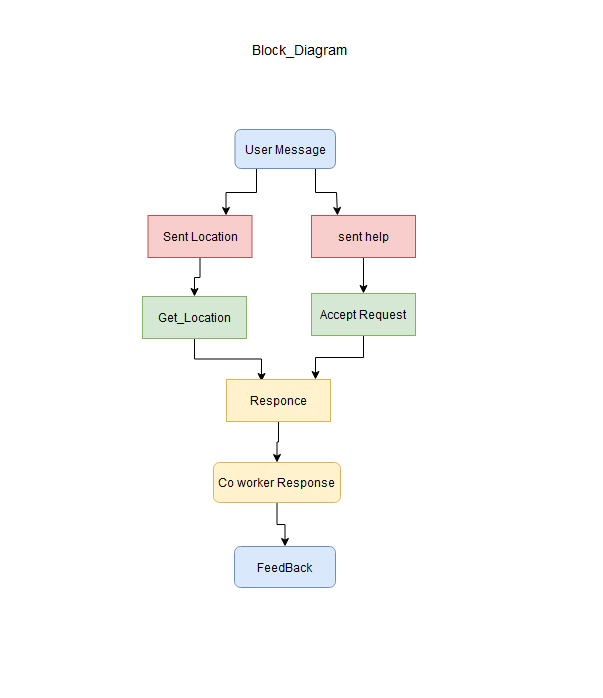
\includegraphics[width=0.8\textwidth]{Block_Diagram.png}

\section{Project Schedule}
\paragraph{First, I have to implement the idea about how actually people get into troble. Then need a specific place where they cna connected by a large area of agent who actually can help. Time is very important for solving a problem in a specific area. So. Govt. service holder can review actually what happends and how to solve it. The whole system need to monitorize for ensuring security for  the people}

\subsection{Gantt Chart}
\paragraph{Gantt Chart have to devided by 4 section.Project , Research Planning and Implement}
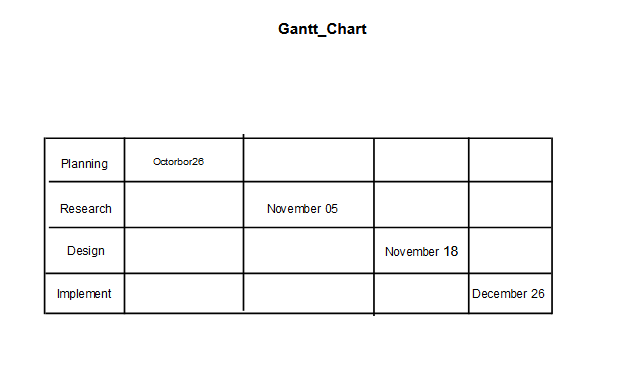
\includegraphics[width=0.8\textwidth]{Gantt_Chart.png}


\subsection{Release Plan/Milestone}
\paragraph{The Plan is mainly for viral any situation in a platform where people can see that and give help or speard news for safety and for the situation. This idea can help the people for awareness at anywhere. This idea can developed a system where any specific area problem can identify by govt services and also people who actually need emergency help by viral the situation. }



\newpage
\section{Functional Requirements}

\begin{tabular}{|p{3cm}||p{3cm}|p{4cm}|p{1cm}  |p{3cm}|  }
 \hline

 \multicolumn{5}{|c|}{Functional  Requirement} \\

 \hline
Requirement&Functional/Non-Functional Category & Description & Priority & Success criteria\\
 \hline
1.FR001:Site Visit  &Functional&The Site will show how the process works&Very High&The site with show the login,signup and other\\
\hline
2.FR002:SignUP&Functional&The chat system needs to require signup&Very High&Signup page show\\
\hline
 3.FR003:Login&Functional&Login page for chat system&Very High&Login page will show chat help\\
\hline
 4.FR004:Chat System&Funcitonal&Chat system will show the main concept&Very High&Chat system for whistleblower\\
\hline
5.FR005:Helpseaker SignUp &Non-Functional&HelpSeaker page for help anywhere by police auth&Middle&Helpseaker signup page \\
\hline
 6.FR006:Forget Login & Functional&Forget page will help to giveaway the account&Very High&Forget page show\\
\hline
7.FR007:Police Verification&Funcitonal&Police verification for the Helpseaker&Very High&Police Verificaton by law enforcement\\
 \hline
\end{tabular}

\section{Data Requirements}
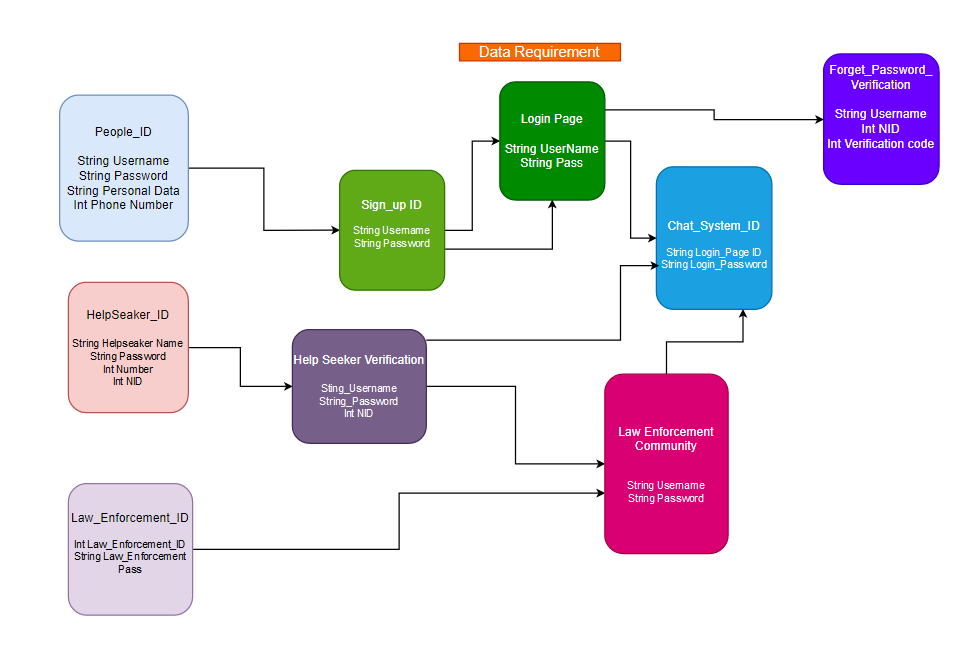
\includegraphics[width=0.8\textwidth]{Data_Requirement.png}



\section{Performance Requirements}
\subsection{Speed and Latency Requirement}

\paragraph{When we use game or use satellite internet, latency can have a big impact on your online experience. In Whistleblower the main page use dynamic programing for get into the chat system. The chat system is the main concept for the idea to help the local people for solving or saving people. So, the system is mainly need real time chat system for this environment. So, we have to use minimum speed and ping for sending and receving data for the exect location. In a
chat platform.120-140ms is optimal for active status. Sending photos and vedios with needs minimum bandwidth which in this system is need some sending bandwidth speed. As a chat system, the medium speed needs to requir for this environment}

\newpage
\subsection{Precision or Accuracy Requirements }
\paragraph{In our country a platform like open chat system is new idea for emergency and accuracy which can help to improve less crime in almost everywhere. This platform require a 
simple easy accuracy for any people for sending text or location for help and the complexity of this system is much faster for the server.}
\subsection{Capacity Requirements}
\paragraph{Capacity requirement meets the full capacity of the system. Ths platform meets the full requirements for emergency help with the people. 
The server gives proper response because  the backend development. The froentend platform is also very fast }

\section{Dependability Requirements}
\subsection{Reliability Requirements}
\paragraph{The Whistleblower system gives a real time solution in a open chat system which can monitored by the law enforcement agency 
which can solve and give a proper solution by given access. This system is robustly help the local people if they have face a problem by bad kind of people. And in emergency they can share their locaiton and ask for helpseaker. The helpseaker also can help them by verify theirselves in law enforcement. So in reality this can be a future solution for vital news and solution. The testing can improve the reliability requirement like subdomain, auth, cross-site for the system. The more test in the system, the better solution for the platform.}

\subsection{Availability Requirements }
\paragraph{The availability in this system is very independent. Every people can use this system as their life saving or any problem solution. This platform is based on division wise traking location for viral situation or any other problems that we face in our daily life. People can use the whistleblower page for give some information which can monitor by law enforcement, helpseaker and any other people in the viral area.
 They can also ask in the chat platform if they want some valuable information and someone can help as a helpseaker}

\newpage
\subsection{Robustness or Fault-Tolerance Requirements }
\paragraph{This system helps to  resist the problem that people facing in the street or any place which we can see in those days in both men and women.
So , in this emergency situation vital solution needs to concern at any location. Now, suppose a women gets harrash in public place. Someone see that and post in whistleblower page.Their will be 
no fault tolerance for viral the system  cause law enforcement always monitor the problem for finding the solution. And it any fault problem post, then punishment will be require with the nid profile.So less tolerance can not be 
ensure in this system.
}

\subsection{Safety-Critical Requirements}
\paragraph{This platform is more safety for local people because their will be no platform abusement for the law enforcement and helpseaker. The police can also help in this problems. So safety critical requirement are less in whistleblower
 chat system.In this system almost every women gets in problem in many place. So helpseaker can asked for help by giving their identity for ensuring the need for help.Safety is more important at any place in our country. Chances for solution is 
widely in this system. Critical situaltion of this platform are most reliable for the people of our county.}

\newpage
\section{Maintainability and Supportability Requirements}
\paragraph{Maintanance requirement}
\subparagraph{Maintainability is the valuable plan for a system. In this project maintain is the most important thing for covering the situation.
Because In a system like open chat system and monitor by law enforcement agents, their will a chance to get hack or system loss by social engineering.
So, the testing needs to be performed in a sequence way so that can not be hacked by the others.}

\paragraph{Supportability requirement}
\subparagraph{Supportability need to require for a system. In this platform law enforcement agent can a hugh amount for supporting the system.They can track anyone if their is any problem.
Law enforcement support can help for data analyst also.In every year submitted problem, disclose and other critical problem might be survey for support and control over by this process.}

\paragraph{Adaptability Requirements}
\subparagraph{The adaptability requiremt need to focus on mission-driven planning for the system. Component based system so that 
it can be implement when it need to update. This adaptibility can be focus on code requirement where developer can help to upgrade and build the system. In this term coding implementation is important for future.}
\paragraph{Scalability or Extensibility Requirements}
\subparagraph{For scalability or extension we can use this system into other platform or mobile operator services. This can be more efficient if people use the cell emergency services for the emergency help. And another thing that people need this system into more feasible like one tap help or location sending message.}


\newpage
\section{Security Requirements}

\paragraph{Access Requirements}
\subparagraph{For every system, data is important for everyone. So access must be secure with a sequence security assurance for the environment.
Each access needs to require with cryptography for storing or accessing the platform. weather it is require for the local people , but their will be focused on law agencies so that they can serve the services
to the local people . Accessing local's data for helping is nessessary for this system. So it wiil be a security process for the platform.
}
\paragraph{Integrity Requirements}
\subparagraph{In data integrity requirement, there will three key attributes:Completeness, accuracy and consistency.A good database will enforce data integrity whenever possible.If the system enforces data integrity, it will prevent the user from making these mistakes.
So, we need to }
\paragraph{Privacy Requirements}
\subparagraph{the privacy requirement must subsantiate this system's compliance with security fundamental privacy.
The fastest way to private and secure in open platform is to secure and implement section wise lookup and extra security for the law enforcement services.
Component -based represents a significant advance towards system by plugging independent and reusable components.So , it makes proper security system.}
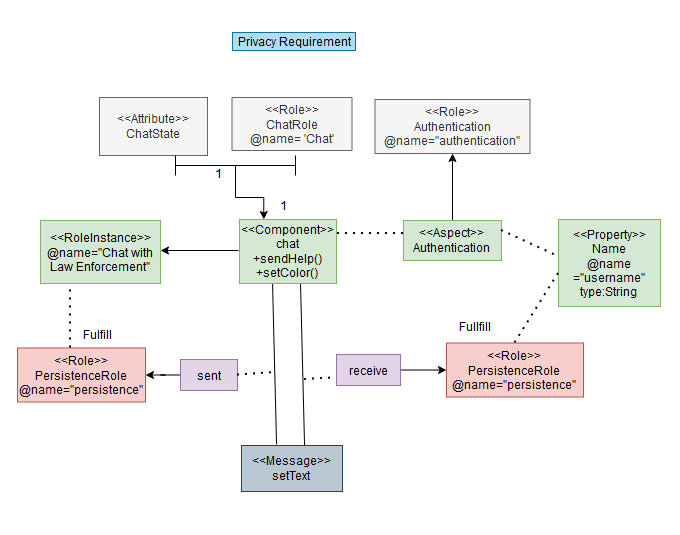
\includegraphics[width=0.8\textwidth]{Privacy_Requirement.png}




\newpage

\section{Security Requirements}
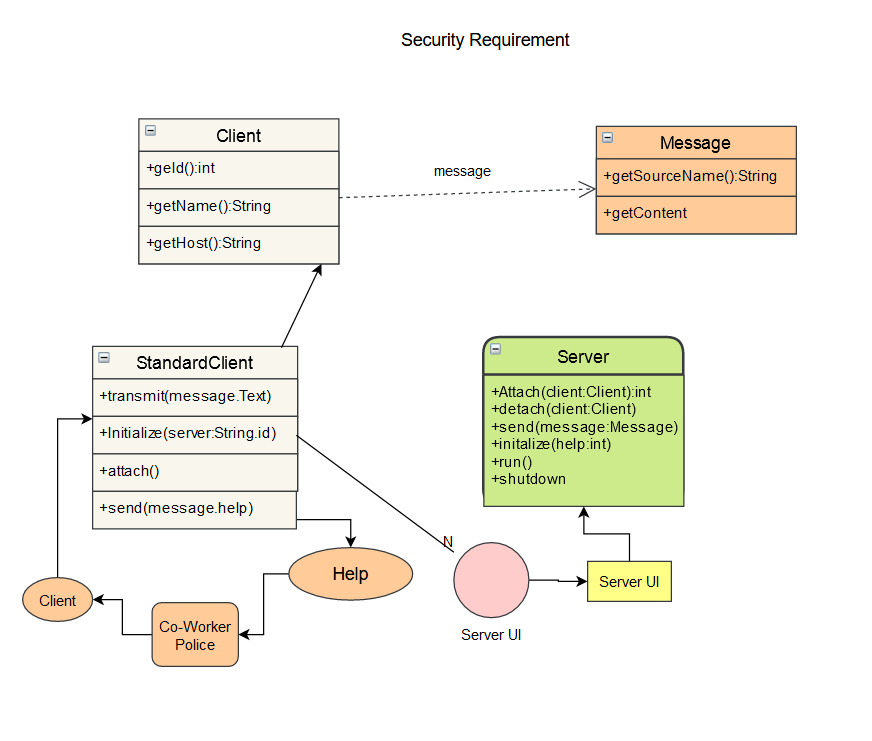
\includegraphics[width=0.8\textwidth]{Security_Requirement.png}
\subsection{It security requirement people need to sent help request in a secure way so that the person don't know the alert and can capture by the law enforcemnt agent , police or co-worker.the goad in security requirement is to keep on the request in track as much as possible}




\paragraph{Ease of Use Requirements}
\subsection{Ease of use requirements need user interface must be familiar to user and need  to follow a single set of rules for the user and the co-worker 
so that they can easily  found by the UI and law enforcement can track them into a secure system.}


\paragraph{Personalization and Internationalization Requirements}
\subsection{It can entails customization related to open source emergency helpline chat system or other system that require people's security so that localization and other different country people can also take the advantages of it.}

\paragraph{Understandability and Politeness Requirements}
\subparagraph{The understandability of this system is easy and more politeness for the user and the co worker. It use  the minimal possibility when the user need help at any place and any where the given location is shared the co worker can notify this.This can made more politeness for the environment}


\paragraph{Accessibility Requirements}
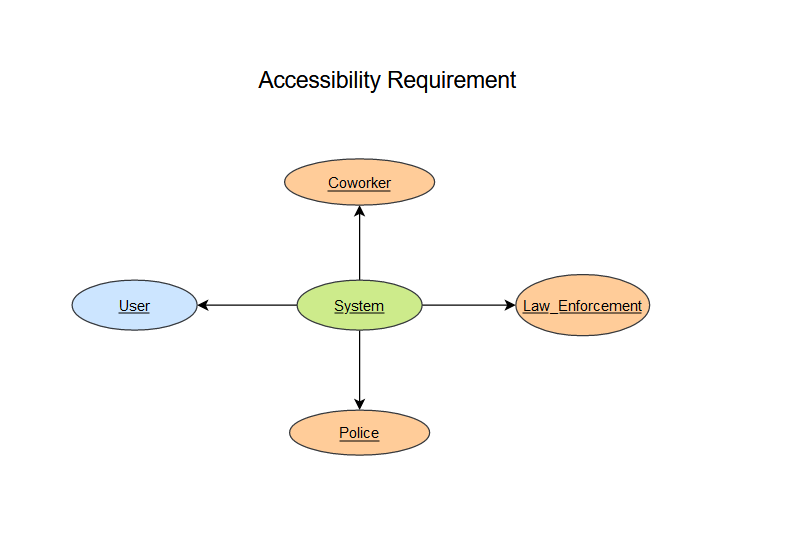
\includegraphics[width=0.8\textwidth]{Accessibility_Requirement.png}




\newpage
\paragraph{User Documentation Requirements}
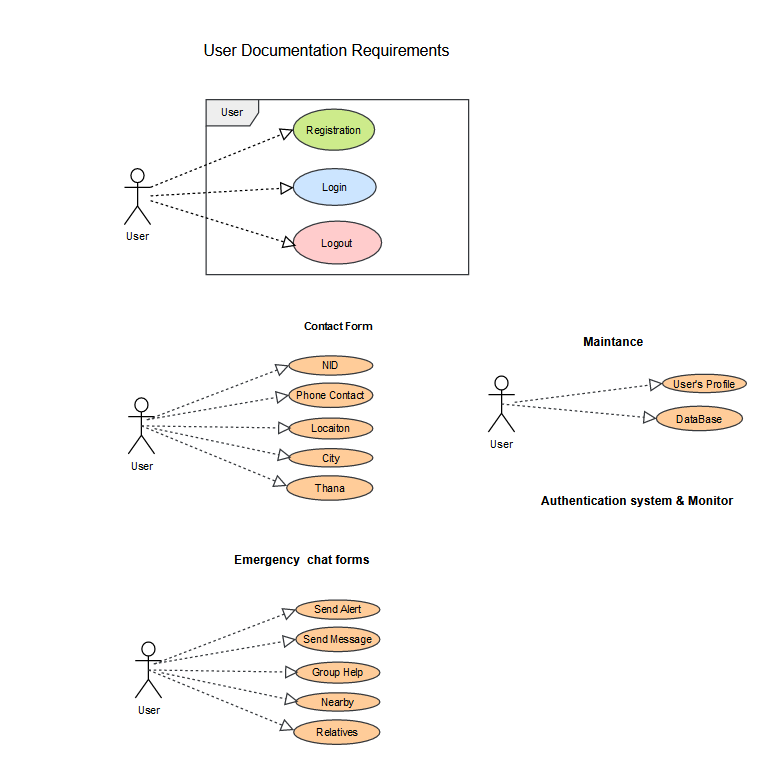
\includegraphics[width=0.8\textwidth]{User_Documentation_Requirement.png}

\paragraph{Training Requirements}
\subparagraph{The training requirement should be  be for the development side and also for the police and co-worker because all are inter connected to the law enforcement and they will always monitoring their server and users.So, the best way is to train both developer and the co-worker who can help 
themselves and the maintaining the system.  }




\newpage
\section{Operational and Environmental Requirements}
\paragraph{The operational and environmental requirement  must need to clear the concept of the database , project scheduling and other more 
security requirement so that the data can be secure and traceble to track the location.}




\newpage


\section{SYSTEM ANALYSIS}


\section{Use Case Diagram}
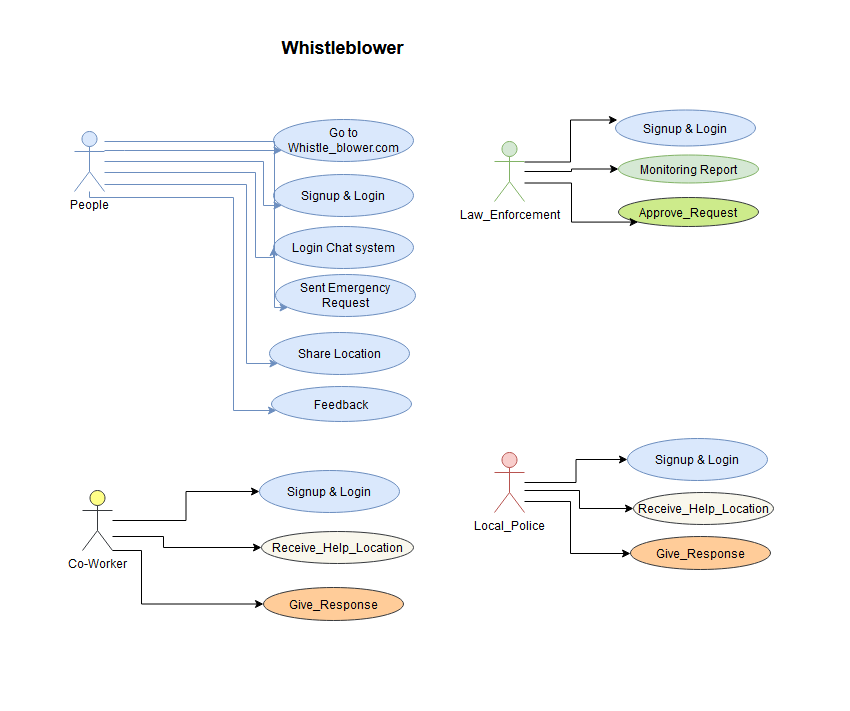
\includegraphics[width=0.8\textwidth]{Use_Case_Diagram.png}
\paragraph{Use Case Description}


\section{Activity Diagram}
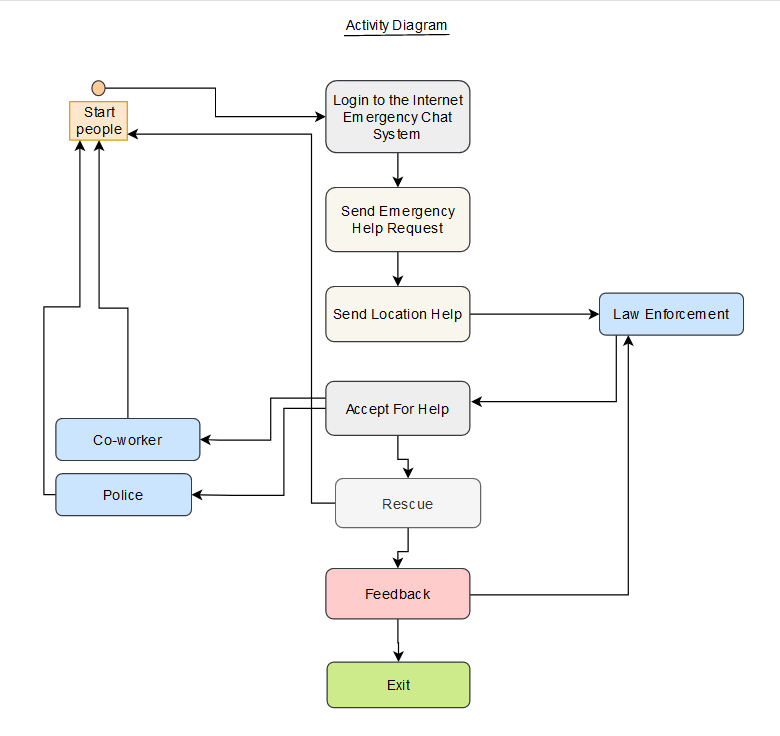
\includegraphics[width=0.8\textwidth]{Activity_Diagram.png}


\section{System Sequence Diagram}
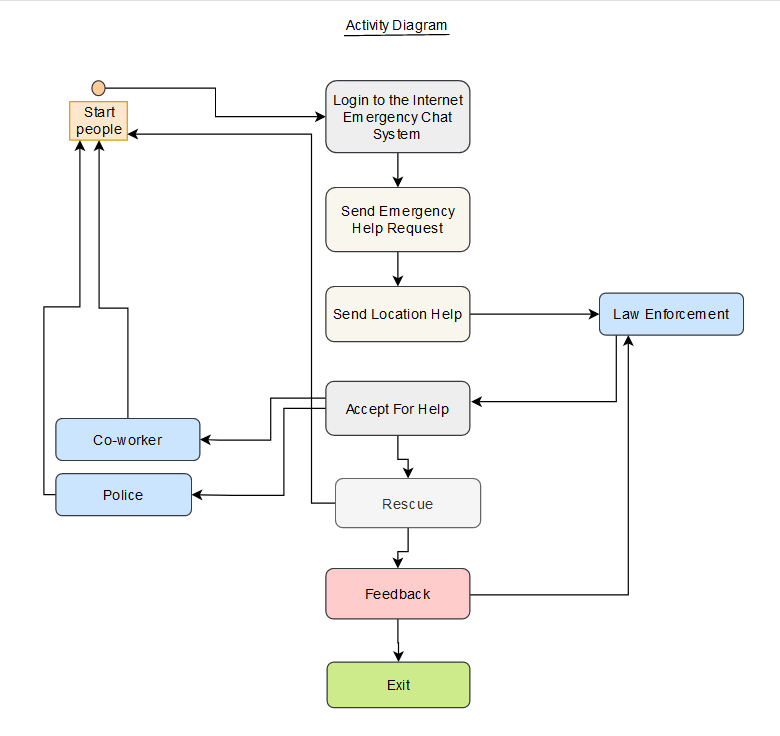
\includegraphics[width=0.8\textwidth]{Activity_Diagram.png}


\newpage
\section{System Design Specification}
\paragraph{Responsibilities Collaboration (CRC) Cards}
\paragraph{Sequence Diagram}


\paragraph{Class Diagram}
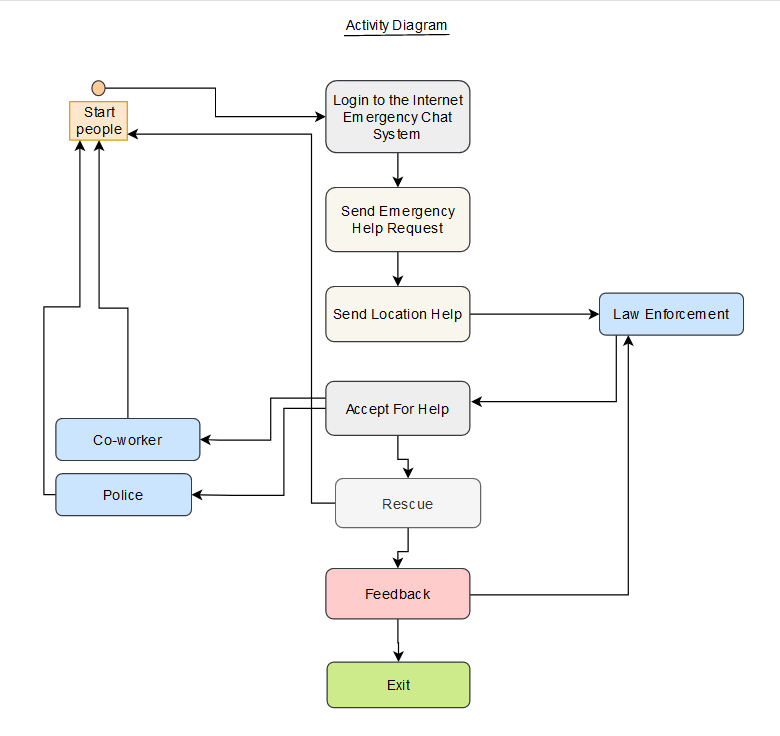
\includegraphics[width=0.8\textwidth]{Activity_Diagram.png}


\paragraph{Database Design Diagram}
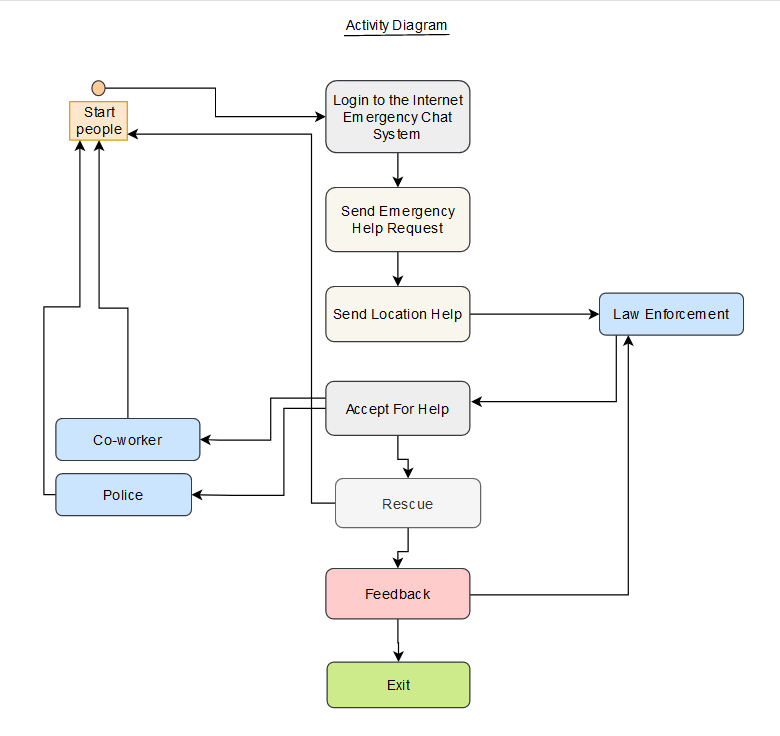
\includegraphics[width=0.8\textwidth]{Activity_Diagram.png}


\paragraph{Development Tools and Technology}
\subsection{User Interface Technology}
\section{Implementation Tools and Platforms}


\newpage
\section{USER MANUAL}


\paragraph{type A user}
\subparagraph{The A type user is the local customer who can use the system for their safety.}

\paragraph{type B user}
\subparagraph{The B type user is the Co worker and the police who can track the request and sent the help for connect the user. }

\paragraph{type C user}
\subparagraph{The c user is the law enforcement who can manage all the system and get connection wiht user and co worker.}

\newpage
\section{PROJECT SUMMARY}
\subparagraph{The project is a milestone for the people of this country . We faced a lot of problems where people facing their problem everyday life. If we can 
solution with proper way by everyone. Then the govt can upgrade the working process and we can be more strong then other country and can grow a economical place.Hence their a possibility of every solution that makes }
\paragraph{Critical Evolution}
\subparagraph{The solution can be given by the person who is connected to the database or the local user. Someone need special help and they need in critical situation. So , this service is about critical emergency moment for the session of our country}

\paragraph{Limitations}
\subparagraph{In every system their's still limitations , In this environment some limitation can be faced like network need to connect in phone.So the phone needs to connected to the platform. In high emergency situation, viral moment need capture at any time. If it can not capture ,the evidence can not be post to the 
right moment.}

\paragraph{Obstacles and Achievements}
\subparagraph{}


\paragraph{Future Scope}
\subparagraph{The Future scope is a chance to decrease harrasement and violation , specially Eve teasing and road haressment . And with full evidence people and govt can see the real problem and give a solution for the problem . Hence , it may be a right term for the future scope. }


\end{document}


